\ylDisplay{Peegeldused} % Ülesande nimi
{Tundmatu autor} % Autor
{piirkonnavoor} % Voor
{2006} % Aasta
{P 7} % Ülesande nr.
{1} % Raskustase
{
% Teema: Valgusõpetus
\ifStatement
Juku näeb peeglist hõõglambi kujutist (suunas A). Sama lambi kujutist märkab ta ka peegli ees olevalt peegeldavalt lauapinnalt (suunas B). Konstrueerige lambi asukoht eraldi lehel oleval joonisel.
\begin{center}
	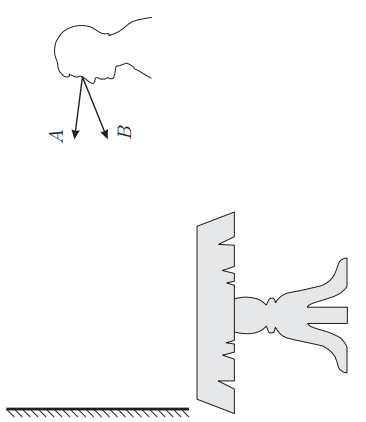
\includegraphics[width=0.5\linewidth]{2006-v2p-07-yl.PNG}
\end{center}
\fi

\ifHint
Lambi asukoha saab määrata kahe peegeldunud sirge lõikepunktiga. Esiteks tuleb pikendada suunas A lähtuvat kiirt ning see peegeldada peegeltasapinnalt vastavalt peegeldumisseadustele. Teiseks tuleb pikendada suuna B lähtuvat kiirt ning peegeldada seda nii laualt kui ka peegeltasapinnalt.
\fi


\ifSolution
Õigel lahendusel saab punkte peeglil toimuva peegelduse õige kujutamise eest; laual tominud peegelduse õige kujutamise eest; peeglil toimunud teise peegelduse õige kujutamise eest, kui kiir B ja peeglilt lambile suunduv kiir on enam-vähem paralleelsed; lambi asukoha leidmise eest, kui lamp asub kahe peeglist tuleva kiire lõikumispunkt.
\begin{center}
	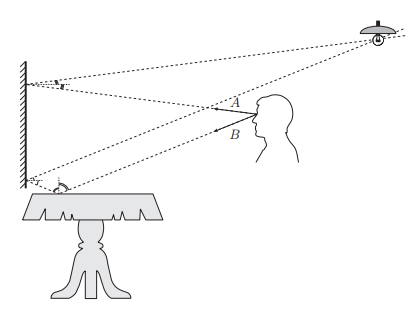
\includegraphics[width=0.5\linewidth]{2006-v2p-07-lah.PNG}
\end{center}
\fi
}
